\documentclass[landscape]{extarticle}
\usepackage[utf8]{inputenc}\usepackage[T1]{fontenc}
\usepackage[spanish,es-noshorthands,es-noquoting]{babel}
\usepackage[a3paper,landscape,margin=1.3cm]{geometry}
\usepackage{graphicx,xcolor,tcolorbox,array,tabularx}
\tcbuselibrary{skins}
\definecolor{az}{HTML}{24618C}\definecolor{ro}{HTML}{C0392B}
\definecolor{ma}{HTML}{8A4B2A}\definecolor{ve}{HTML}{2E7D43}
\definecolor{gris}{HTML}{4A4A52}
\newtcolorbox{tarjeta}[2]{colback=#1!5,colframe=#1,fonttitle=\bfseries\LARGE,
  title=#2,left=3.5mm,right=3.5mm,top=2.5mm,bottom=2.5mm,boxrule=1.4pt,arc=2.5mm,
  width=\linewidth,height=9.5cm,valign=top}
\newcommand{\filas}[1]{\large\begin{tabularx}{\linewidth}{@{}X>{\raggedleft\arraybackslash}p{4.3cm}@{}}#1\end{tabularx}}
\setlength{\parindent}{0pt}\pagestyle{empty}
\begin{document}

{\fontsize{40}{44}\selectfont\bfseries DaVinci Paddle Boat}\hfill
{\LARGE\bfseries Reto EIA 2027 · Marymount}\\[2mm]
{\Large\color{gris} Barco de paletas en madera, cortado a láser · tres unidades}\\[3mm]
{\color{gris}\hrule height 2.5pt}\vspace{6mm}

\noindent
\begin{minipage}[t]{0.305\textwidth}
  \vspace{0pt}
  \begin{center}
  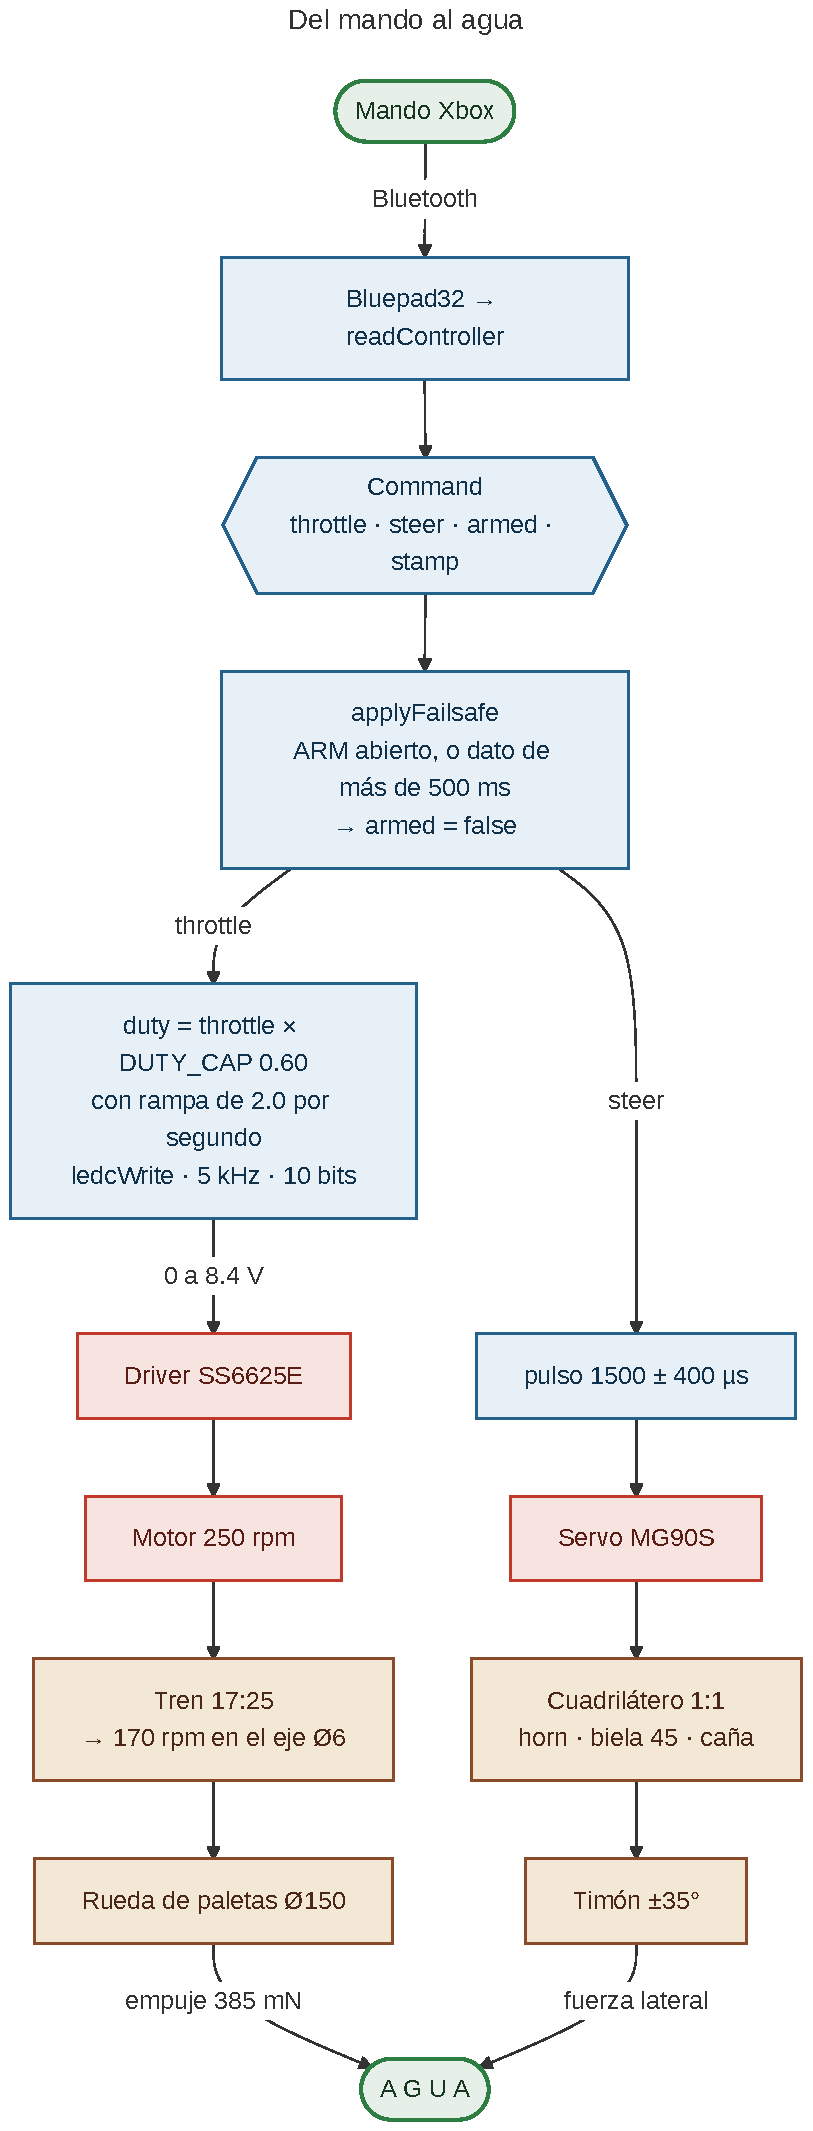
\includegraphics[height=22.6cm]{cadena-mando-agua.pdf}
  \end{center}
\end{minipage}\hfill
\begin{minipage}[t]{0.665\textwidth}
  \vspace{0pt}
  \begin{minipage}[t]{0.485\linewidth}\begin{tarjeta}{ma}{CASCO}
    \filas{
      Eslora × manga × puntal & 370 × 140 × 70 \\
      Material & contrachapado 4 mm \\
      Astilla muerta & 45° \\
      Calado / francobordo & 55.9 / 14.1 mm \\
      GM & +25.2 mm \\}
    \vspace{1.5mm}{\small\color{gris} Los costados son paneles \textbf{planos}: la quilla
    sube a proa para que la madera no tenga que doblarse fuera de plano.}
  \end{tarjeta}\end{minipage}\hfill
  \begin{minipage}[t]{0.485\linewidth}\begin{tarjeta}{ro}{PROPULSIÓN}
    \filas{
      Motor & 250 rpm · 6 V \\
      Engranajes & 17 : 25, módulo 2 \\
      Rueda de paletas & Ø150, 6 palas \\
      Velocidad & 0.75 m/s \\
      Número de Froude & 0.39 \\}
    \vspace{1.5mm}{\small\color{gris} Los engranajes van en \textbf{madera laminada}, como
    pide la rúbrica. Ø150 es el tamaño que agota lo que este casco puede dar.}
  \end{tarjeta}\end{minipage}

  \vspace{7mm}

  \begin{minipage}[t]{0.485\linewidth}\begin{tarjeta}{az}{GOBIERNO}
    \filas{
      Pala del timón & 24 × 44 mm \\
      Compensación & 20 \% \\
      Recorrido & ±35° \\
      Varillaje & cuadrilátero 1:1 \\
      Par en el servo & 0.017 kg·cm \\}
    \vspace{1.5mm}{\small\color{gris} Brazos iguales da paralelogramo, y el timón gira
    \textbf{exactamente} lo que gira el servo. Sin tablas de calibración.}
  \end{tarjeta}\end{minipage}\hfill
  \begin{minipage}[t]{0.485\linewidth}\begin{tarjeta}{ve}{CONTROL}
    \filas{
      Cerebro & ESP32-WROOM-32E \\
      Mando & Xbox por Bluetooth \\
      Failsafe & 500 ms sin enlace \\
      Modo autónomo & tramo recto de 15 s \\
      Tope de PWM & 0.60 \\}
    \vspace{1.5mm}{\small\color{gris} El barco no se mueve si no está \textbf{armado}: el
    interruptor y el failsafe mandan sobre cualquier orden del mando.}
  \end{tarjeta}\end{minipage}

  \vspace{9mm}
  {\color{gris}\hrule height 1.2pt}\vspace{3mm}
  {\normalsize \textbf{Tres barcos, dos motores distintos.} Dos llevan motor de 250 rpm
  (engranajes 17:25) y uno de 170 rpm (21:21). Las dos combinaciones suman 42 dientes, así
  que dan la misma distancia entre centros: \textbf{lo único distinto entre los tres barcos
  son dos engranajes}.\\[2mm]
  {\color{gris} Límite del reto: 400 mm de eslora y 300 de manga. Usados: 397 y 276.}}
\end{minipage}

\end{document}
